\section{Problem 5: BGP Routing}
\subsection{part 1}

We use notation S to represent source and D for destination.

\textbf{First example:} S first sends a file to D through routers A and B. The path is described as S-A-B-D. However, when D try to send a file back to S follow the reverse path, it finds that the link from A to S is highly congested. Therefore, to avoid congestion, D sends file to B and then routes the file around A, say B-E-S. In such case, asymmetric routing happens.

\textbf{Second example:} assume S is D's client and D is A's client. S and A are peers. The relationship is presented in Figure

\begin{figure}[h]
    \centering
    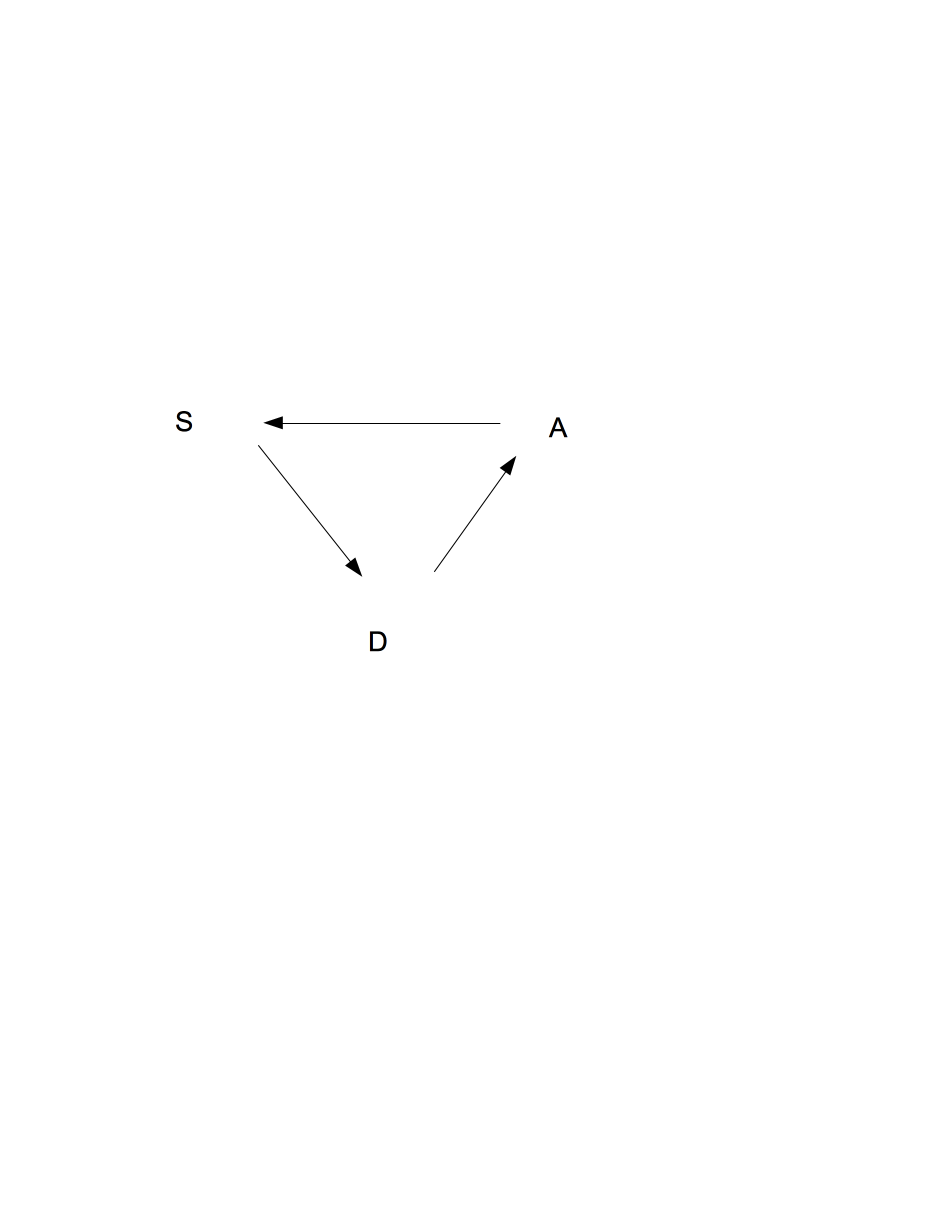
\includegraphics[trim = 0 360 40 90mm, clip, width=0.8\textwidth]{p5.png}
    \caption{Client customer relationship. Arrow points from client to provider.}
    \label{fig:p5}
\end{figure}

When S try to send a file to D, it will choose to route through A instead of directly send the file to D since it prefers peer. The route will be S-A-D. When D try to send a file to S, it will choose to send it directly to S since S is its customer. And we have an asymmetric routing situation.

%%%%%%%%%%%%%%%%%%%%%%%%%%%%%%%%%%%%%%%%%%%
\subsection{part 2}

\begin{enumerate}
\item One possible attack is that both E and F not broadcasting D's information. If, as shown in the problem that D is only connected to E and F, then D will not be able to receive ant data packets from any other domain. In other words, D is being blocked. In order to limit the impact of D from getting blocked and get aware of the situation sooner, a server located in domain other than E and F could be used to periodically sends data packets to D to see if D is able to receive any. If D is not receiving any packets from the server, then clearly D is being attacked.
\item Another possible attack is that E broadcasts an invalid route for E to send data packets to another domain, say A. In such case, E could get data packets from D and discard them and the data packets will be lost. To protect D from such attack, Secure BGP could be applied to prevent such routing manipulation. Secure BGP validates attributes in BGP update messages between ASes through the use of digital signatures and associated public key certificates.
\item The third possible attack is a DDoS attack from E to D by sending huge amount of data packets, such as BGP updates, to overload D. What D could do to protect itself against this attack is running a filtering algorithm at its gateway which is connected to E. The filtering algorithm identifies the prefixes and restricts the amount of BGP updates gets sent into D in a fixed period of time.
\end{enumerate}
